\documentclass[a4paper]{article}
\usepackage[margin=2cm]{geometry}
\usepackage{amsmath, amssymb, graphicx, float, forloop, longtable}
\graphicspath{{../result}{../report/media}}

\title{Analytical Scan Result Interpretation}
\author{PokMan Ho}

\begin{document}
\maketitle

\section{P+B vs P-only systems by harvest rates}
\begin{itemize}
    \item System carbon distribution:
    \begin{itemize}
        \item log total carbon distribution: all categories are significant (p-val = 0.0000 (4d.p.)) under Wilcox test
        \item log organic carbon \& log yield flux: non-significant in harvest rate 0.3 $day^{-1}$ (p-val = 0.0563 (4d.p.)) and 0.4 $day^{-1}$ (p-val = 0.7878 (4d.p.))
        \item distribution shape \& statistical summaries of organic carbon and yield is exactly the same; graphs are shifted left for histograms from organic carbon to yield while it is downwards in the line charts: $log yield flux = log organic carbon + log harvest rate$
    \end{itemize}
    \item Wilcox test showed a peak in p-val around harvest rate = 0.4
\end{itemize}

\begin{table}[H]
    \centering
    \caption{Statistical summary of all Wilcox test on organic carbon pool / yield flux by harvest rate}
    \begin{tabular}{l|rrrrrrrrrr}\hline
        rate & 0.1 & 0.2 & 0.3 & \textbf{0.4} & 0.5 & 0.6 & 0.7 & 0.8 & 0.9 & 1 \\\hline
        W $\times 10^3$ (3 s.f.) & 659 & 505 & 511 & \textbf{541} & 485 & 426 & 438 & 404 & 366 & 346 \\
        p-val (4 d.p.) & 0 & 0.0003 & 0.0563 & \textbf{0.7878} & 0.0037 & 0 & 0 & 0 & 0 & 0 \\\hline
    \end{tabular}
    \label{tab:pVal}
\end{table}

\section{General features of biological parameters}
\begin{table}[H]
    \centering
    \caption{Table of biological parameter effect on carbon distributions}
    \begin{tabular}{llll}\hline
        Var & definition & effect for P-only & effect for P+B \\\hline
        $e_{PR}$ & non-respired P carbon fraction & $\uparrow$ with $\downarrow$ rate & slight $\uparrow$ (total), stable (org-C) \\
        $e_P$ & P carbon fraction to biomass & stable & stable (total, org-C) \\
        $g_P$ & P growth rate & $\uparrow$ with $\downarrow$ rate [bumpy] & slight $\uparrow$ (total), stable (org-C) \\
        $a_P$ & P intraspecific interference & $\downarrow$ with $\downarrow$ rate & $\downarrow$ with $\downarrow$ rate (total), stable (org-C) \\
        $e_{BR}$ & non-respired B carbon fraction & stable & U-shaped (total), $\downarrow$ (org-C) \\
        $e_B$ & B carbon fraction to biomass & stable & slight $\downarrow$ (total), $\downarrow$ with $\downarrow$ rate (org-C) \\
        $g_B$ & B clearance rate & stable & $\downarrow$ with $\downarrow$ rate [slight bumpy] (total, org-C) \\
        $m_B$ & B death rate & stable & \begin{tabular}{@{}l}
            stable [slight bumpy] (total), \\
            $\uparrow$ with $\downarrow$ rate [bumpy] (org-C)
        \end{tabular}  \\
    \hline\end{tabular}
    \label{tab:varEffect}
\end{table}

\begin{itemize}
    \item change of P biological features would affect B but not vice versa (effect of indirect trophic level?)
    \item the ``fraction" category: $e_{PR}$ $\uparrow$, $e_P$ no effect, $e_{BR}$ \& $e_B$ $\downarrow$
    \item the ``rate" category: $g_P$ \& $m_B$ $\uparrow$, $a_P$ \& $g_B$ $\downarrow$
    \item P+B feasibility limit found not on harvest rate ($x$) within parameter range but on $e_{BR}$ (limit $\approx$ 0.9, independent from $x$)
\end{itemize}

\section{Low harvest rate: 0.1 $day^{-1}$}
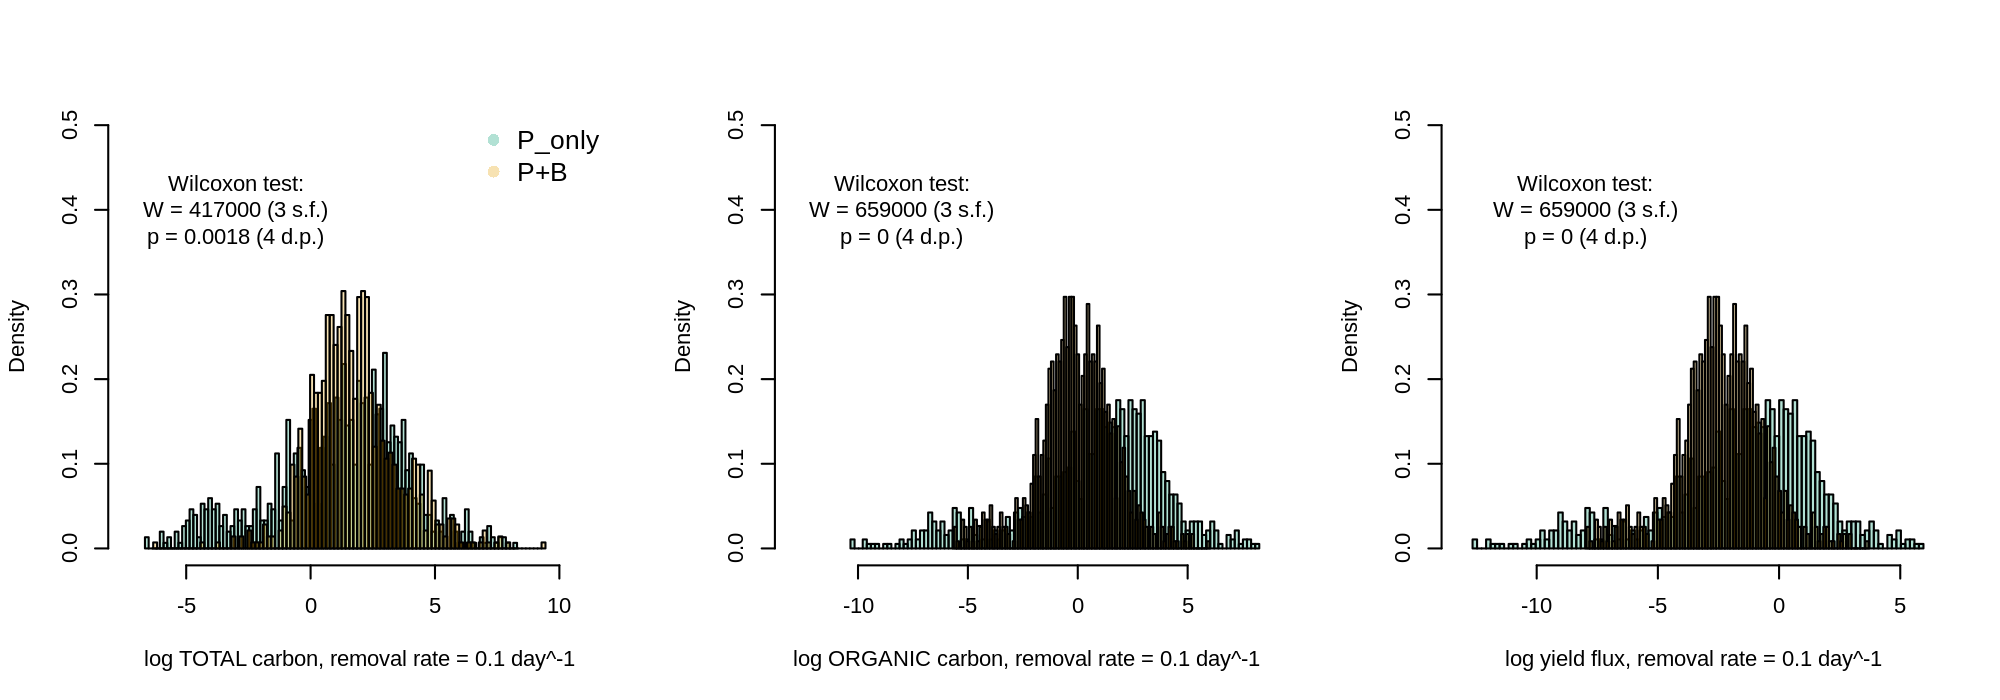
\includegraphics[width=\linewidth]{../result/sys_01.png}\\
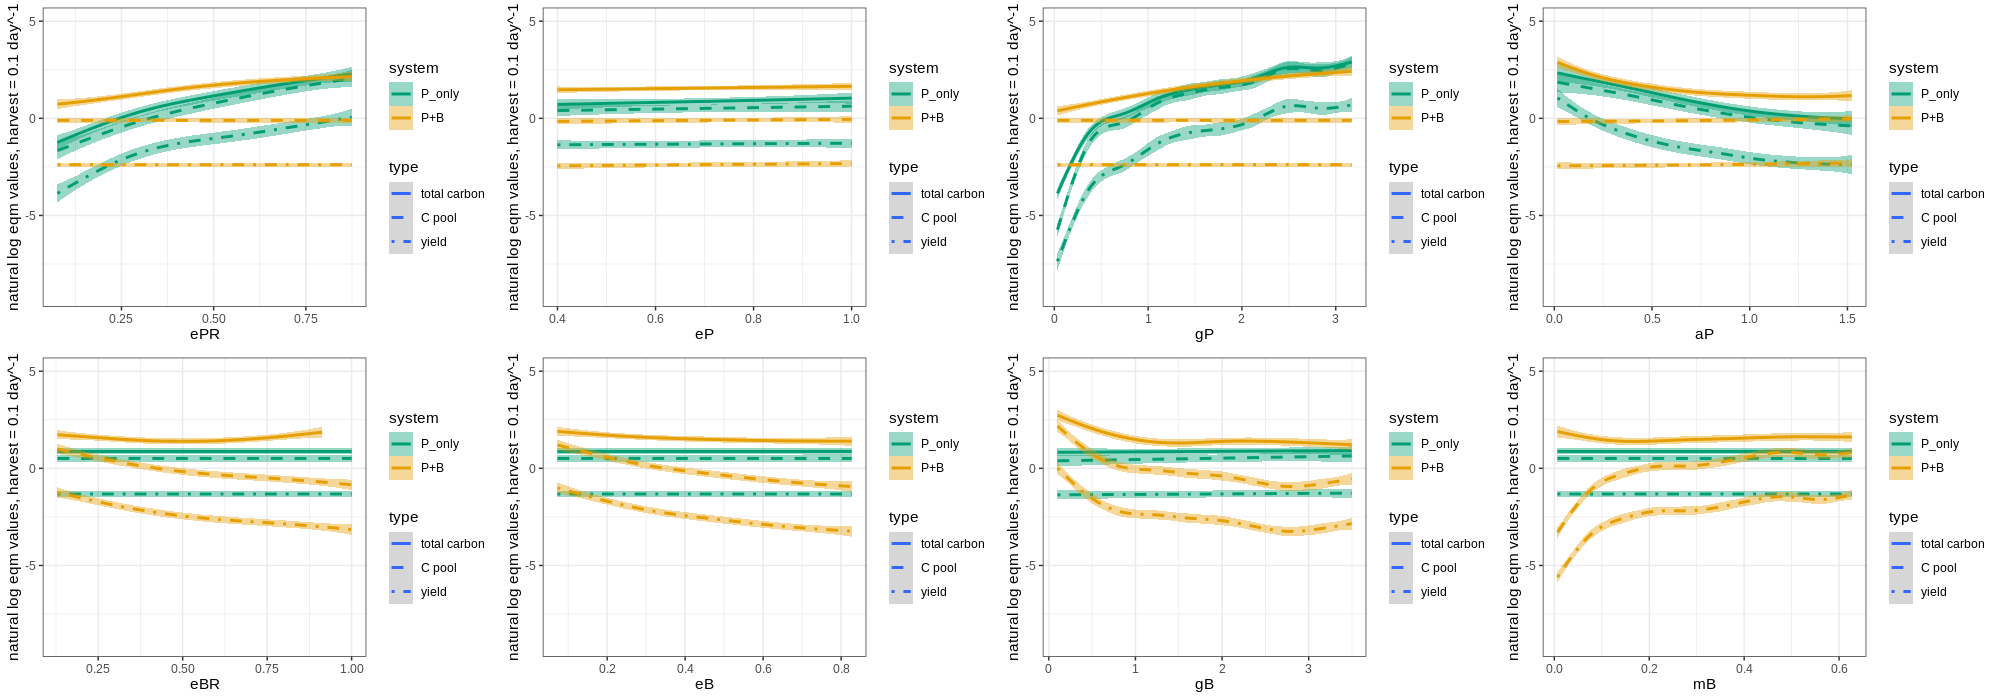
\includegraphics[width=\linewidth]{../result/var_01.png}\\

\subsection{total carbon}
\begin{itemize}
    \item 95\% distribution usually don't overlap between P+B \& P-only systems
    \item highest overlap occur in $g_P$ but at lower end the difference is much larger than when viewed from other parameters' perspectives
    \item overall distribution (left histogram) has similar peak size but still with statistical significance
\end{itemize}

\subsection{org-C / yield}
\begin{itemize}
    \item crossover in biological parameters are usually in lower side of parameter ranges (except $m_B$)
    \item more values of P-only systems $>$ P+B ones
    \item overall distribution (middle histogram) having P-only higher
\end{itemize}

\section{Medium harvest rate: 0.4 $day^{-1}$}
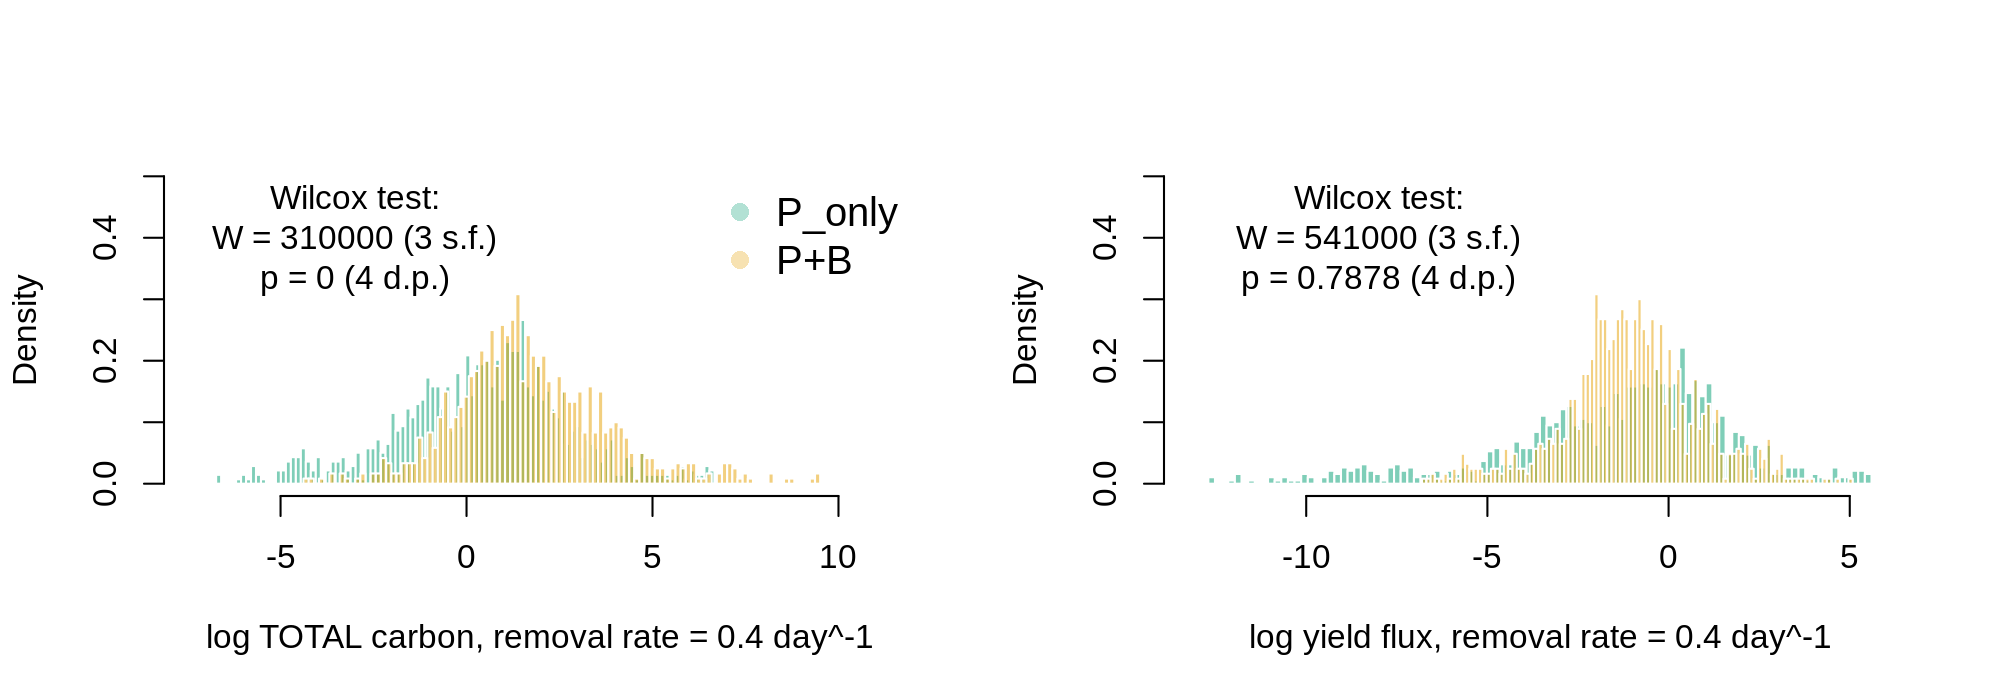
\includegraphics[width=\linewidth]{../result/sys_04.png}\\
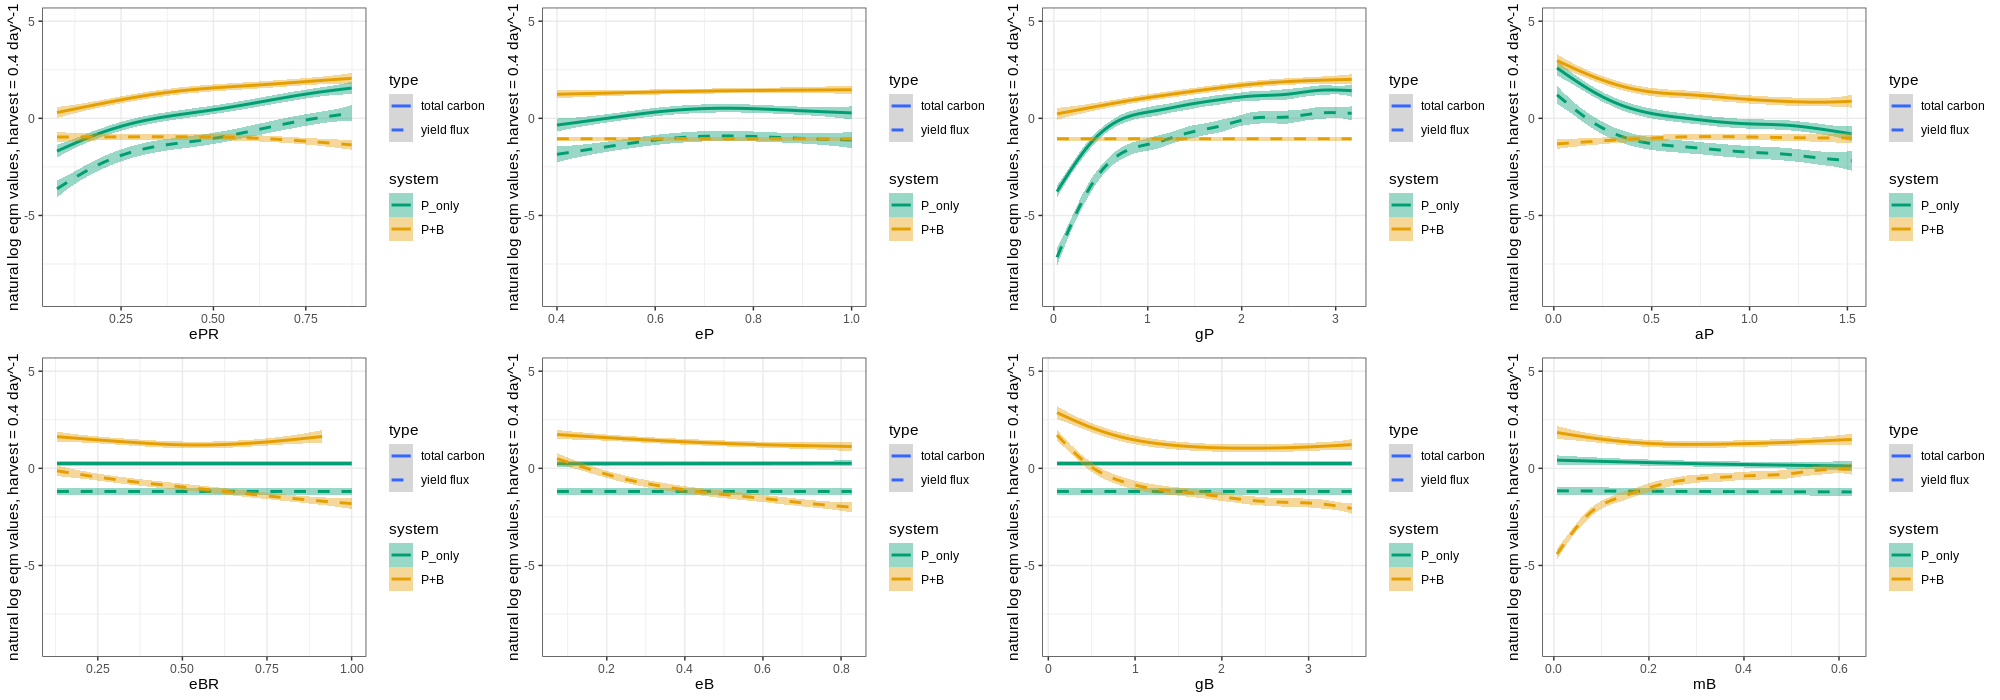
\includegraphics[width=\linewidth]{../result/var_04.png}\\

\subsection{total carbon}
\begin{itemize}
    \item 95\% distribution mostly don't overlap between P+B \& P-only systems
    \item highest overlap occur at end of $e_{PR}$ and start of $a_P$ ranges but at the opposite ends the difference is high
    \item overall distribution (left histogram) is similar but still with statistical significance
\end{itemize}

\subsection{org-C / yield}
\begin{itemize}
    \item $e_P$ have P+B \& P-only systems almost overlapping each other
    \item $e_{BR}$ have P+B \& P-only systems crossing but neither ends are having high differences compared with distributions from other parameters' perspectives
    \item $g_B$ \& $m_B$ have P+B \& P-only systems with high difference at small values but as values increases both systems come close to each other and not showing big difference at high end of the range
    \item overall distribution (middle histogram) having different shapes (P-only having a long low-end tail) but they're not having statistical difference
\end{itemize}

\section{High harvest rate: 1 $day^{-1}$}
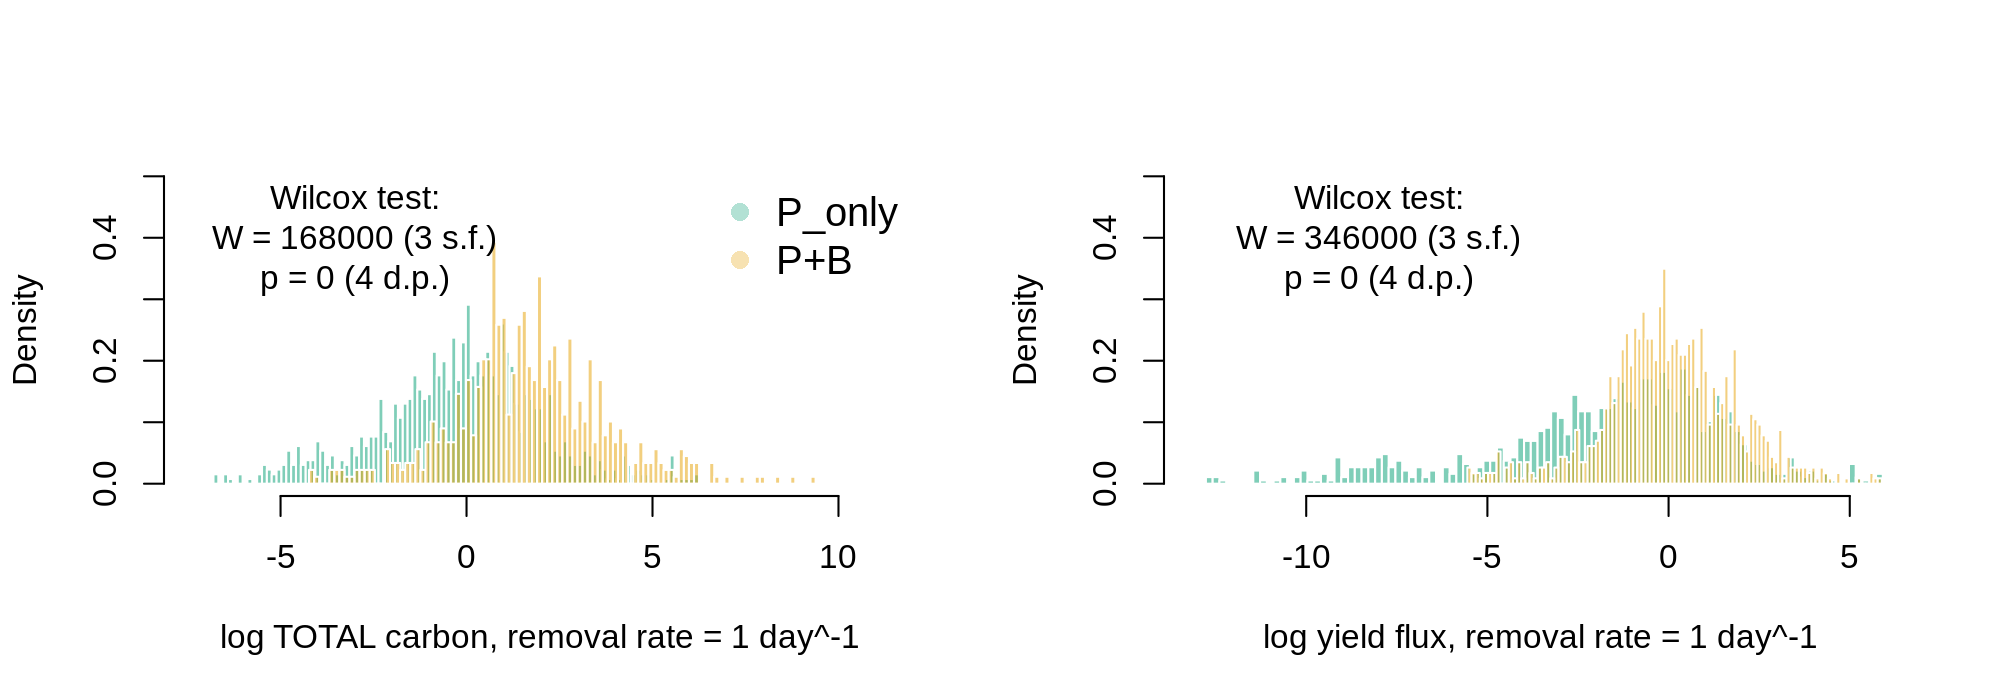
\includegraphics[width=\linewidth]{../result/sys_10.png}\\
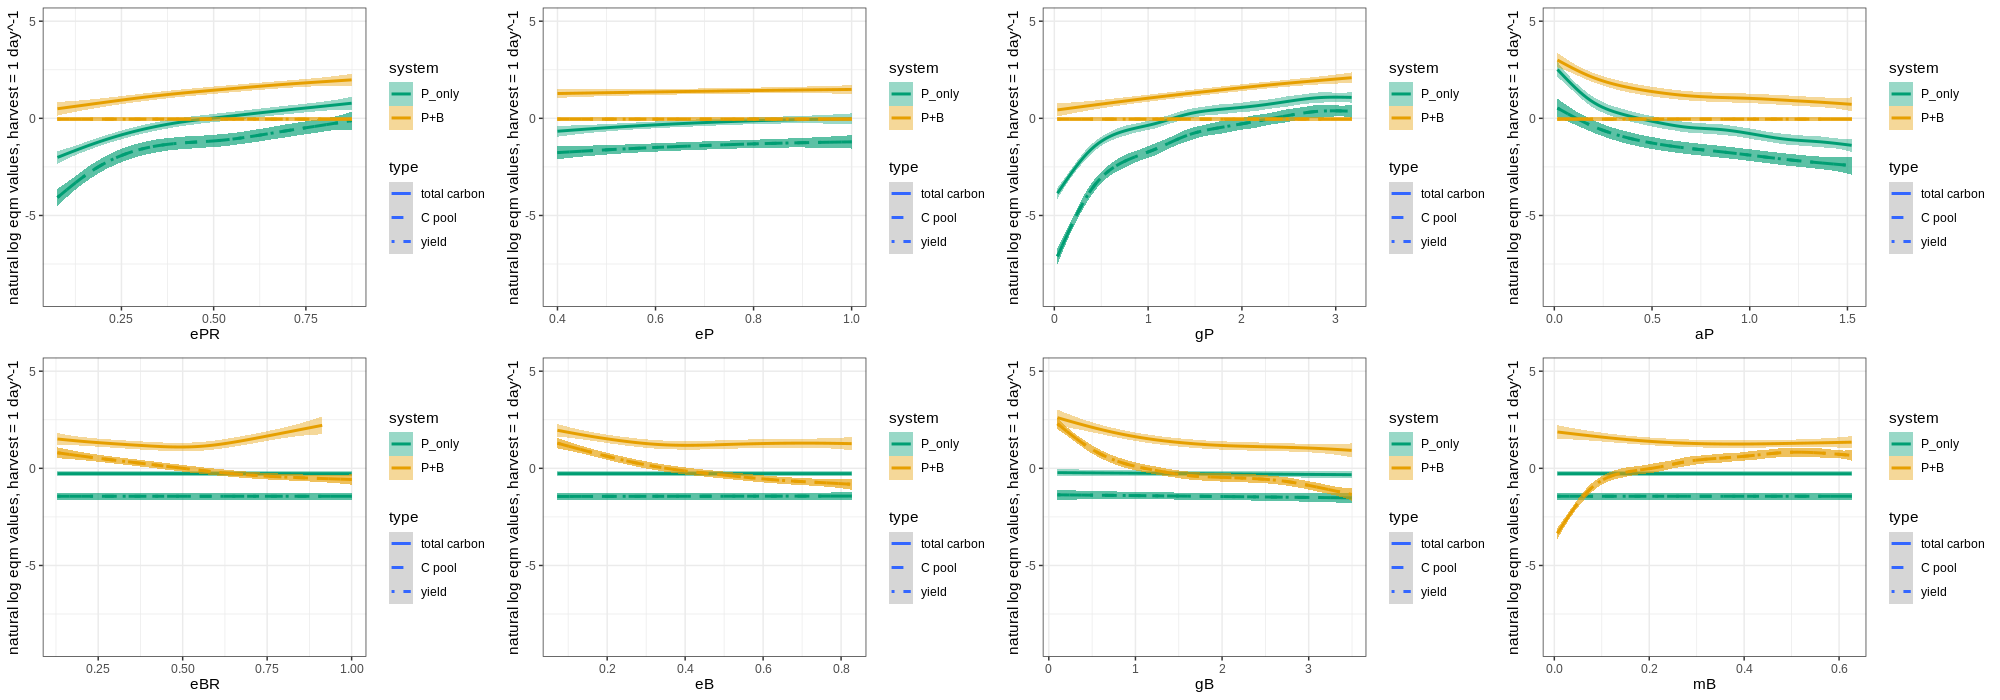
\includegraphics[width=\linewidth]{../result/var_10.png}\\

\subsection{total carbon}
\begin{itemize}
    \item 95\% distribution don't overlap between P+B \& P-only systems
    \item highest difference happen in low $g_P$ and lowest difference in low $a_P$ regions respectively
    \item overall distribution (left histogram) has P+B distribution peaked on the right of the P-only one
    \item due to the stability in the P+B result (small 95\% interval on each solid line and across the 8 parameters), peak density of P+B higher than that of P-only
\end{itemize}

\subsection{org-C / yield}
\begin{itemize}
    \item log(yield)|$_{x=1}$ = log(org-C) + log($x$) = log(org-C)
    \item change of P parameters do not have observable effect on P+B log value (in smaller $x$ values fluctuated more)
    \item change of B parameters gave more consistent effect across parameter ranges
    \item most P+B values are higher than that of P-only
    \begin{itemize}
        \item $e_{PR}$, $g_P$, $g_B$ got (close to be) overtaken by P-only distributions
        \item $e_P$, $e_{BR}$, $e_B$ always had their distributions higher than P-only
        \item $a_P$, $m_B$ had P+B overtook P-only values at small parameter values
    \end{itemize}
    \item overall distribution (middle histogram) having P+B higher in central peak density; P-only has a wider spread in log carbon pool size
\end{itemize}

\end{document}